
\documentclass[conference]{IEEEtran}
\usepackage{cite}
\usepackage{graphicx}
\usepackage{amsmath}
\usepackage{enumerate}
\usepackage{xcolor}
\usepackage{pgfplots}
\usepackage{tikz}
\usepackage{listings}
\usepackage[linesnumbered]{algorithm2e}
\usepackage{tikz}


\begin{document}

\title{BUMPER: A Tool to Cope with Natural Language Search of Millions Bugs and Fixes}


\author{\IEEEauthorblockN{Mathieu Nayrolles, }
\IEEEauthorblockA{Software Behaviour Analysis (SBA) Research Lab\\
ECE, Concordia University\\
Montreal, Canada\\
m\_nayrol@ece.concordia.ca}
\and
\IEEEauthorblockN{Abdelwahab Hamou-Lhadj}
\IEEEauthorblockA{Software Behaviour Analysis (SBA) Research Lab\\
ECE, Concordia University\\
Montreal, Canada\\
abdelw@ece.concordia.ca}}

% make the title area
\maketitle

% As a general rule, do not put math, special symbols or citations
% in the abstract
\begin{abstract}
  In recent years, mining bug report (BR) repositories has perhaps been one of the most active software engineering research fields. There exist many open source and proprietary bug tracking and source code versioning systems that developers and researchers can use to examine bug reports so as to reason about software quality. The issue is that these repositories use different interfaces and ways to access and represent data, which hinders productivity and reuse. To address this, we introduce BUMPER (BUg Metarepository for dEvelopers and Researchers), a common infrastructure for developers and researchers interested in mining data from different (and heterogeneous) repositories. BUMPER is an open source web-based environment that extracts information from a variety of BR repositories and source code versioning systems. It is equipped with a powerful search engine to help users rapidly query the repositories using a single point of access. To demonstrate the effectiveness of BUMPER, we use it to build a large dataset from a variety of repositories. The dataset contains more than one million of bug reports and fixes. Both BUMPER and the dataset are publicly available online at https://bumper-app.com.

\end{abstract}


\IEEEpeerreviewmaketitle


\section{Introduction}

Debugging programs, during their creations or at maintenance time is challenging \cite{Pressman2005} and taxing --- Studies have shown that the cost of software maintenance can reach up to 70\% of the overall cost of the software development process.

When facing a yet unknown bug, one might want to leverage decades of open-source software history in order to find a solution. Indeed, chances are a similar bug or crash has already been fixed somewhere in an open-source project.

However, each open-source project host its data in a different data repository and using different bug tracking and source code management systems. Moreover,   these systems have different interfaces to access data.
The data are not represented in a uniform way either.
This is further complicated by the fact that bug tracking tools and code versioning systems are not necessarily connected.
The former follows the life of the bug itself and not its fixes, which are managed by the latter.
As a general practice, developers create a link between the bug report system and the source versioning tool by either writing the bug \#ID in their commits message or add a link towards the Changeset as a comment in the bug report system.

As a result, one would have to search the source code versioning system repository to find candidate solutions.
 Moreover, developers mainly use classical search engines that index specialized sites such as StackOverflow.

However, specialized sites are organized in the form of question-response where one explain his problem and gets answers from the community. While the answers are often accurate and precise, they do not leverage the history of open-source software that has been shown to provide useful insight to help with many maintenance activities such as bug fixing\cite{Saha2014}, bug reproduction\cite{Chen2013a}, fault analysis\cite{Nessa2008}, etc.

In this paper, we introduce BUMPER (BUg Metarepository for dEvelopers and Researchers), a web-based infrastructure that can be used by software developers and researchers to access data from diverse repositories using natural language queries in a transparent manner, regardless of where the data were originally created and hosted.

The idea behind BUMPER is that it can connect to any bug tracking and source code versioning system and download the data into a single database.
BUMPER uses a web-based interface that allows users to search the aggregated database by expressing queries through a single access point.
This way, users can focus on the analysis itself and not on the way data is represented or where it is located.

BUMPER supports many features including: (1) the ability to search large data repositories very efficiently using both natural languages and a specialized query language, (2) the mapping between the bug reports and the code involved to fix it, (3) the ability to export the search results in Json, CSV and XML formats.

Finally, we asked developers to solve a bug using habitual habit and using BUMPER. The results indicate that our approach reduces the amount of data-sources to be visited in order to find a suitable solution for the bug at hand and therefore, speeding up the debugging and maintenance processes.

\section{Bumper Components}
\label{sec:Bumper Components}

BUMPER aggregate data from various bug tracking and version control systems that can be efficiently accessed using a web-based interface.
Currently, BUMPER supports 380 projects, more than 100,000 resolved/fixed and with 60,000 changesets from Netbeans and the Apache Software foundation’s softwares.
It can readily be extended to support other systems.
Using BUMPER, software engineers can query multiple repositories and save the data in various formats including Json, CSV, and XML for further analysis.

\subsection{Bumper architecture}
\label{sub:Bumper architecture}


BUMPER relies on a highly scalable architecture composed
of two Virtual Private Servers (VPS), hosted on a physical
server.
The first server handles the web requests and
runs three distinct components: Pound, Varnish, and NginX.
Pound is a lightweight open source reverse proxy program
and application firewall.
It also serves to decode https to request to http.
Translating an https request to http allows us to save the https decryption time required on each step.
Pound also acts as a load-balancing service for the lower levels.
The translated requests are then handled by Varnish.
Varnish is an http accelerator designed for content-heavy and dynamic websites.
It caches requests that come in and serves the Web requests from the cache is the cache is still valid.
NginX (pronounced engine-x) is a web-server that was developed with a particular focus on high concurrency, high performances, and low memory usage.
The second VPS also uses Pound for the same reasons and SolrCloud.
SolrCloud is the scalable version of Apache Solr where the data can be separated into shards (e.g chunk of manageable size).
Each shard can be hosted on a different server, but still indexed in a central repository.
Hence, we can guarantee a low query time while exponentially increasing the data.
Finally, Lucene is the full text search engine powering Solr.
This highly scalable architecture allows Bumper to serve requests under.5 second, in average.

\subsection{BUMPER Metadata}
\label{sub:BUMPER Metadata}

Figure~\ref{fig:bumper-metamodel}  shows the core BUMPER metamodel, which captures the common data elements used by bug tracking and control version systems.
An issue (task) is characterized by a date, title, description, and a fixing time.

\begin{figure*}
  \centering
  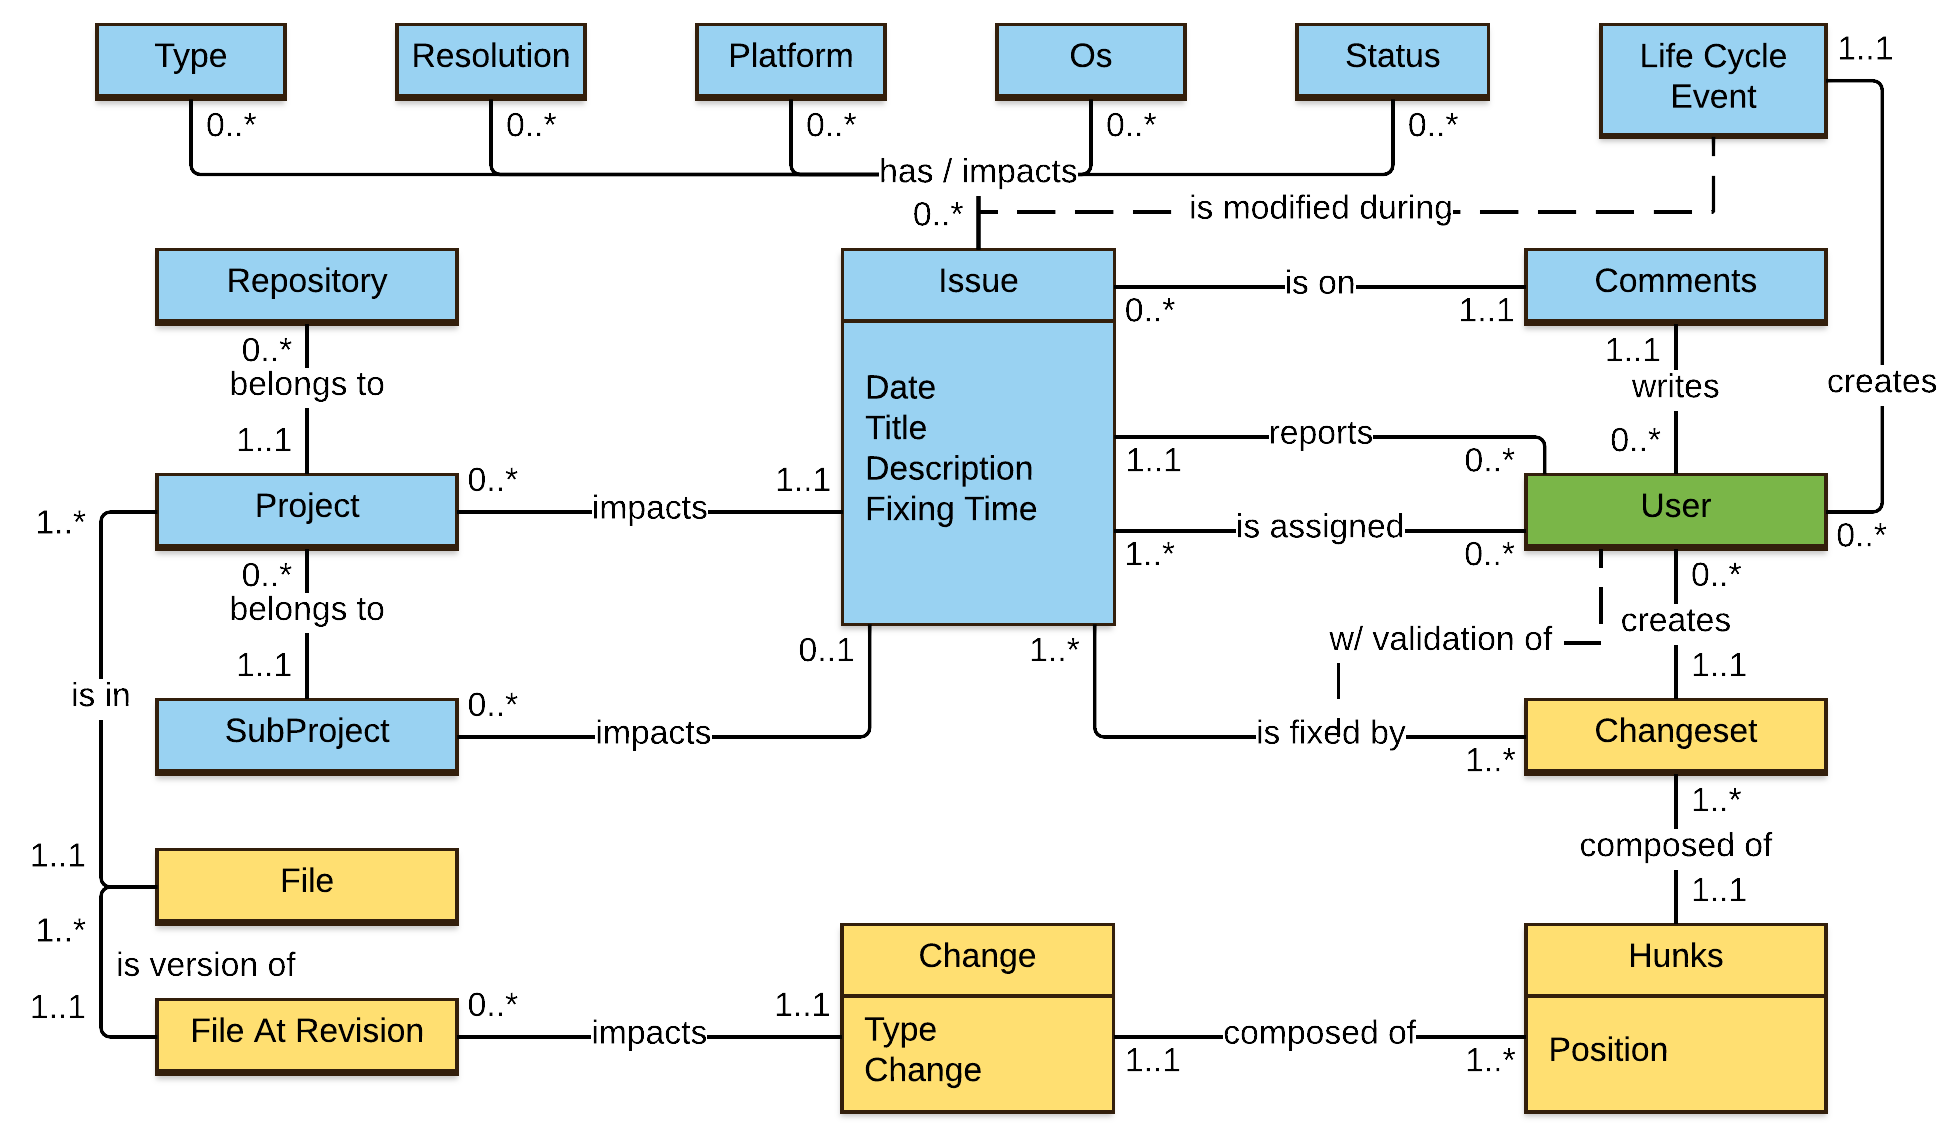
\includegraphics[width=0.7\textwidth]{media/Bumper-Model.png}
  \caption{BUMPER Metamodel\label{fig:bumper-metamodel}}
\end{figure*}

Issues are reported (created) by and assigned to users.
Also, issues belong to a project that is in a repository and might be composed of subprojects.
Users can modify an issue during life cycle events which impact the type, the resolution, the platform, the OS and the status.
Issues are resolved (implemented) by changeset that are composed of hunks.
Hunks contain the actual changes to a file at a given revision, which are versions of the file entity that belongs to a project.
In addition, BUMPER has different indexes over the data in order to provide results in an efficient way.
First of all, each feature of bug reports and bug fixes (number of files, number of hunks, etc.) have their own index.
Furthermore, BUMPER has data indexes over the project name, the sub-project name, the programming language, etc.
Finally, two major indexes are built upon the concatenations of all the textual fields of the bug report and all the textual field (source code included) of a bug fix.
They are named report\_t and fix\_t, respectively.
These indexes are used when querying bug reports or bug fixes using natural language.
Indexes can also be found in relational database management system (RDBMS).
Most modern RDBMS uses binary trees to store indexes that keep data sorted and allow searches, insertions, and deletion in a logarithmic time.
Nevertheless, an RDBMS can use only one index per table at the same time.
This said, an RDBMS chooses only one index within the available ones--based on statistics--and uses it to complete the request.
It is highly probable that thousands of records have to be scanned before the RDBMS finds the ones that match the query, especially if there is a union or disjunction of records.
Unlike a traditional RDBMS, BUMPER relies on Apache Lucene and uses compressed bitsets to store indexes.
Bitsets are one of the simplest--and older--data structure that contain only 0 and 1.
BUMPER supports binary operations like intersection, AND, OR and XOR that can be performed in a snap for even for thousands and thousands of records.
As an example, if we wish to retrieve bug reports that contain the words null pointer exception and have a changeset containing a try/catch, a binary intersection will be performed between the two sets of documents, which is much faster than selecting bug reports that match null pointer exception first and then checking if they have a changeset containing a a try/catch as in the case of an RDBMS.
This technique comes with a high overhead—comparing to an RDBMS--for index update, but, in practice, information retrievals are orders of magnitude faster.
In our case, we want to provide a fast access to decades of open source history.
We periodically update (at night) our indexes when sufficient amount of new data has been downloaded from the bug tracking and source versioning systems BUMPER supports

\subsection{Bumper Query Language and API}
\label{sub:Bumper Query Language and API}

BUMPER supports two query modes: basic and advanced.
The basic query insert users' inputs (YOUR TERMS) in the
following query:

\begin{equation}
\begin{split}
~~(type:``BUG"~AND~report_t:``YOUR~TERMS"~\\
~~AND~-churns:0)
\end{split}
\end{equation}



The first part of the query matches all bug reports
(type:"BUG") that contain YOUR TERMS in the report\_t index
(report\_t:"YOUR TERMS").
Finally, it excludes bug reports that
do not have a fix (-churns:0).
The result of this subquery will be
merged with the following:

\begin{equation}
\begin{split}
~~OR~(\{!parent~which=``type:BUG"\}type:~\\
~~``CHANGESET"~AND~fix_t:``YOUR~TERMS"
\end{split}
\end{equation}

This query selects all bugs' changeset--using a parent-child
relationship $(\{!parent~which=``type:BUG"\}~type:
  ``CHANGESET")$ -- and that contain YOUR TERMS in the fix\_t
  index (fix\_t:``YOUR TERMS").
Finally, the results of the two
previous queries will be added to the following subquery:

\begin{equation}
\begin{split}
  OR~(\{!parent~which=``type:BUG"\}\ \\
~\{!parent~which=``type:CHANGESET"\}\\
~type:``HUNKS"~AND~fix_t:``YOUR~TERMS")
\end{split}
\end{equation}

The query selects all the hunks that are child of changsets and
grand-child of bug report $ (\{!parent~which=``type:BUG"\}
  \{!parent~which=``type:CHANGESET"\}~type:``HUNKS")$
and that
contain YOUR TERMS in the fix\_t index.
The intent of this composed query is search efficiently for
YOUR TERMS in bug reports, commit messages and source
code all together.
The advanced query mode allows users to write their own
query using the indexes they want and the unions or disjunctions
they need.
As an example, using the advanced query mode, one
could write the following:

\begin{equation}
\begin{split}
  (type:``BUG"~AND~report_t:``Exception"~\\
~~AND~(project:``Axis2"~OR~project:``ide")~\\
~~AND~(reporter:``Rich"~OR~resolution:``fixed")~\\
~~AND~(severity:``Major"~OR~fixing_time:[10~TO~*])~\\
~~AND~-churns:0)
\end{split}
\end{equation}

This query finds all bug reports that contain Exception in the
report\_t index (first line) and belong to the Axis2 or the ide
project (line 2) and have been reported by someone named Rich
or have been fixed as a resolution (third line) and that have a
Major severity or a fixing time greater than 10 days (fourth line)
and have a fix (fifth line).
More examples of the API's usage can
be found at https://bumper-app.com/api.


\subsection{Bumper Data Repository}
\label{sub:Bumper Data Repository}

First, we extract the raw data from bug report management systems of five different open source institutions used in this study: Gnome, Eclipse, Netbeans, Apache Software Foundation and Github.
Each institution is composed of many open source projects: 10, 192, 39, 349 and 250, respectively. Summing up to 840 different open source projects.

The extracted data is consolidated in one database where we associate each bug report with its fix.
The fixes are mined from different types of source versioning system.
Indeed, Gnome, Eclipse and Apache Software Foundation projects are based on Git (or have git based mirrors) while Netbeans uses Mercurial.

Gnome is a free desktop environment, mainly developed in c and c++ by volunteers and paid contributors both.

Eclipse and Netbeans are integrated development environments (IDEs) for developing with many programming languages, including Java, PHP, and C/C++.

The Apache Software Foundation (ASF) is a non-profit public charity established in 1999, that provides services and support for many like-minded software project communities of individuals who choose to join the ASF.

Finally, Github is a free web-based Git repository hosting service that allows anyone to create, version and maintain a team development project while using Git as source code management and Github issues as Bug management system.

The characteristics of the five datasets used in this paper are presented in Table~\ref{tab:summary}.
Cumulatively, these datasets span from 2001 to 2014.

\begin{table}[]
\centering
\caption{
RESOLVED/FIXED BUG (R/F BR),  CHANGSETS (CS), AND
PROJECTS BY DATASET}
\label{tab:summary}
\begin{tabular}{c|c|c|c|c}
\textbf{Dataset} & \textbf{R/F BR} & \textbf{CS} & \textbf{Files} & \textbf{Projects} \\ \hline \hline
Gnome            &                 &             &                & 10                \\ \hline
Netbeans         & 53,258          & 122,632     & 30,595         & 39                \\ \hline
Apache           & 49,449          & 106,366     & 38,111         & 349               \\ \hline
Eclipse          &                 &             &                & 192               \\ \hline
Github           &                 &             &                & 250               \\ \hline
Total            &                 &             &                & 840               \\ \hline \hline
\end{tabular}
\end{table}

In summary, our consolidated dataset contains 102,707 bugs, 229,153 changesets, 68,809 files that have been modified to fix the bugs, 462,848 comments, and 388 distinct software tools.
We also collected 221 million lines of code impacted by the changesets, identified 3,284 sub-projects, and 17,984 unique contributors to these bug report systems.

We choose these five datasets because they exposed a great diversity in programming languages, teams, localization, utility and maturity.
Moreover, the used different tools, i.e.
Bugzilla, JIRA, Git and Mercurial, and therefore, Bumper is ready to host any other datasets that used any composition of these tools.

Bumper users can follow the same process to add another
Repositories from various bug tracking and version control
systems such as Eclipse, Mozilla Foundation datasets. The BUMPER architecture can then be used to organize and
access multiple repositories in a unified manner.

\section{Experiments}
\label{sec:Experiments}

In order to assess the efficiency of BUMPER during the debugging / maintenance processes we conduct an online survey in which we present participants with a bug to fix.
Then, we ask them to find a suitable solution of the presented bug online as would have in a classical debugging / maintenance session and repeat the operation using BUMPER.
Finally, participants were asked to report how long it took to find a suitable solution with both methods and to rate their experience using BUMPER.

We presented participants of our online survey\footnote{http://goo.gl/forms/RvYFACkl7a} with the following made up bug\footnote{https://github.com/MathieuNls/bumper-csv}: \textit{When I run the CSVReader with a simple main like this:}

\noindent\begin{minipage}{0.90\linewidth}

  \lstinputlisting[language=Java, firstnumber=1, numbers=right, stepnumber=1,leftmargin=30, label=javabug, caption=Java Bug]{media/bug.java}

\end{minipage}

\textit{I got the following Exception: Exception in thread ``main" java.lang.NullPointerException at CsvFileUtils.readOneLine(CsvFileUtils.java:22) at Main.main(Main.java:11). Can you please fix CsvFileUtils ?}

The solution to this simple bug is straight forward as we only have to add a null check to line 22 of CsvFileUtils\footnote{https://github.com/MathieuNls/bumper-csv/blob/master/src/CsvFileUtils.java}.

Participants were asked to find a code a code snippet that can be slightly modified in order to fix a bug using Bumper and Google.
The goal of the experiment was to compare how fast a suitable fix can be found using Bumper and Google.
Consequently, we asked participant look for a fix online even if they know how to fix.

We send our survey to 20 participant ant got 8 responses (40\%) and asked them to report their experience in terms of time taken to find a fix and webpages browsed.
Participants reported then, when using Google, it took, on average, 6.94 minutes and 7.57 sources to find a fix.
When using Bumper, however, it took only 4.5 minutes and one webpage (i.e. https://bumper-app.com).


\section{Related Works}
\label{sec:Related Works}

Codemine \cite{Czerwonka2013} and Boa \cite{Bizer2011} are two well-known projects that enable the mining and reporting of code repository, including bug report and related fixes.
Both tools, however, will require the download of all the data and process the mining for each installation.

To the best of our knowledge, no attempt has been made towards building an unified and online datasets, from multiple sources, where all the information related to a bug, or a fix can be easily accessed by researchers and engineers in order to leverage decades of historical information.
Providing a unified, online, and easily accessible datasets have been shown to be effective for learning new APIs\cite{Montandon2013,Rahman2013} and BUMPER aims to achieve a similar goal, which is empowering developers by giving access to multiple data repositories that they can use to find how similar bugs have been fixed throughout the history of hundreds of well known software projects.


\section{Conclusion}
\label{sec:conclusion}

In this paper, we presented an online tool named BUMPER (BUg Metarepository for dEvelopers and Researchers) accessible at https://bumper-app.com. BUMPER allows natural language searches in bugs reports, commit messages and source code all together while supporting complex queries and contain 380 projects, more than 100,000 resolved/fixed and with 60,000 changesets that were involved in fixing them from Netbeans and The Apache Software foundation’s software.

The speed of BUMPER allows developers to use it as a way to leverage decades of history scattered over hundreds of software projects in order to find existing solutions to their problems.
Furthermore, users found a solution to a simple bug 40\% faster using Bumper than Google.


\bibliographystyle{IEEEtran}
\bibliography{library}


\end{document}
